\subsubsection{Частотно-временной анализ} 

Аналогично формализации SSA (\myref{link::ssa}), также рассматриваем  второе определение стационарности (\myref{def::signal_stationarity}), предполагающее отношение к сигналу как набору величин, характеризующих некоторый объект на промежутке времени. Ключевой особенностью рассматриваемого в текущем блоке подхода - анализа Фурье - является <<сканирование>> исходных сигналов в частотном пространстве, а не временн\'{о}м, в котором данные изначально представлены. \textbf{Q}: Каким образом осуществляется переход подобного рода? \textbf{A}: Описано далее. Однако помним, что теперь сигнал, будучи характеристикой некоторого объекта может быть непрерывен, что уводит нас от дискретного анализа, как было в случае подхода ARIMA и GARCH (ARFIMA и FIGARCH уже немного залезли в непрерывную область с точки зрения лагов), к непрерывному. Обратный переход делается при построении и рассмотрении алгоритма Быстрого Преобразования Фурье (Fast Fourier Transform - FFT) (\myref{link::fft}), где для корректной работы алгоритма как такового требуется переход к дискретности. 

Из непрерывности сигнала следует факт, что теперь сигнал - это некоторая функцию $f: \R \to \R$, от переменной $t$ - время. Более того, пока что не делаем никаких предположений относительно поведения $f(t)$, то есть она, конечно, непрерывна, иначе разрыв характеризовался бы потерей соединения с записывающим устройством, но о наклонах, изгибах и так далее предположения пока что не выдвигаются.

Теперь переходим непосредственно к блоку анализа Фурье, где объясняется принцип и необходимость перехода к частотному (только частотному, а не частотно-временному) пространству.

\subsubsubsection{Анализ Фурье} \label{link::fourier_analysis}
\\\\
\indent По изначальному подходу, сигнал $f(t)$ - это некоторая функция, то есть ее можно пытаться чем-то приближать. Конечно, далеко не всякую функцию можно аппроксимировать, однако пока что оставляем математическую строгость за кадром и просто пробуем. Но в таком случае из чего-то сложного как исходный сигнал, получаем что-то более простое, но поддающееся анализу, значит, мы раскладываем имеющуюся $f(t)$ на простые составляющие. Замечаем, что в первом приближении для этого должны быть выбраны простые функции, которые легко поддаются анализу. В таком случае, задаемся вопросом~\textbf{Q}: Можно ли как-то представить функцию вида $f(t)$ (исследуемый непрерывный сигнал) в виде конечного или бесконечного наложения синусоид (под синусоидой понимается как косинус, так и синус). \textbf{A}:~1)~Замечаем, что существует неточность: почему именно синусоиды? \textbf{Q}:~Почему нельзя взять иной набор функций, на которые раскладывается сигнал? \textbf{A}: Любой набор взять нельзя, однако при определенных условиях подобный подход приводит к рассматриваемому далее Wavelet анализу (\myref{link::wavelet_analysis}). На данный момент останавливаем рассуждения на  упоминании синусоид. Изначально было отмечено \cite{mipt2021string}, что струна - это тонкая и гибкая нить, способная совершать колебания при условии фиксированных концов как раз на основе синусоидальных форм. Причем по всей длине струны всегда умещается конечное количество волн. Это обеспечивается условием закрепленности струны на обоих концах. 

Самая простая форма колебания струны называется "гармоникой". Отсюда и происходит второе название анализа Фурье - гармонический анализ. Таким образом, формализуя исходную задачу, получаем выражение (\ref{equation::fourier_approximation}). Отмечаем, что факт того, как данное выражение изначально получено находится за областью, исследуемой в настоящей работе. Следовательно, предполагаем, что подобная форма разложения в ряд Фурье была <<угадана>>. 
\begin{equation} \label{equation::fourier_approximation}
	f(t) = \frac{a_0}{2} + \sum_{k = 1}^{\infty} a_k\cos(k \omega t) + b_k\sin(k \omega t)
\end{equation}
\indent Однако, несмотря на вольность предположений, далее совершенно строго находим для данного разложения все необходимые коэффициенты. Более того, отмечаем, что пока не было введено никаких предпосылок относительно $f(t)$, но далее они потребуются.

Пусть исходный сигнал $f(t)$ является периодическим с периодом $T$, тогда, основываясь на знаниях из Линейной Алгебры об ортогональных векторах, по аналогии вводим операцию <<измеряющую степень>> ортогональности функций~\cite{penn2016orthogonal}. В итоге получаем:
\begin{equation}
	p = \int_0^T g(t) f(t) \; \text{d}t
\end{equation}
\indent Далее вычисляем данную меру для выбранных в качестве базисных функций $\cos(\cdot)$ и $\sin(\cdot)$. Если $p \ne 0$, то вся проводимая операция не может быть названа разложением по базисным функциям. В силу того, что под <<синусоидой>> подразумевается как $\sin(\cdot)$, так и $\cos(\cdot)$, вычисляем меру $p$ для каждого из четырех возможных вариантов их комбинаций.
\begin{enumerate}
	\item $\sin(k\omega t), \sin(l \omega t): k, l \in \N, \omega \in \R^+$.
	\begin{equation}
		p = \int_{0}^T \sin(k\omega t)\sin(l \omega t) \; dt =
		\left\{
		\begin{array}{rl}
			0 & \text{, } k \ne l\\
			T / 2 & \text{, } k = l
		\end{array}
		\right.
	\end{equation}
	
	\item $\cos(k\omega t), \cos(l \omega t): k, l \in \N, \omega \in \R^+$.
	\begin{equation}
		p = \int_{0}^T \cos(k\omega t)\cos(l \omega t) \; dt =
		\left\{
		\begin{array}{rl}
			0 & \text{, } k \ne l\\
			T / 2 & \text{, } k = l
		\end{array}
		\right.
	\end{equation}
	
	\item $\cos(k\omega t), \sin(l \omega t): k, l \in \N, \omega \in \R^+$.
	\begin{equation}
		p = \int_{0}^T \cos(k\omega t)\sin(l \omega t) \; dt = 0
	\end{equation}
\end{enumerate}
Тогда, опираясь на  выражение (\ref{equation::fourier_approximation}) и умножение его обеих частей на $\sin(k\omega t)$ и $\cos(l \omega t)$, получаем формулы для коэффициентов. Рассматриваем только для $\sin(\cdot)$, так как аналогичным образом получается для $\cos(\cdot)$.
\begin{equation}
	\int_{0}^T f(t) \sin(p \omega t) dt = \int_0^T \sin(p \omega t) \left(\sum_{k = 1}^{\infty} a_k\cos(k \omega t) + b_k\sin(k \omega t) \right) dt
\end{equation}
Однако изменять порядок интегрирования и суммирования, при условии бесконечной суммы, можно только в случае равномерной сходимости ряда. Для настоящего ряда проблем в сходимости не наблюдается \cite{teljacovski2001convergence}, \cite{mipt2004fourier}. Преобразуем выражение, приняв во внимание факт ортогональности функций, описанный выше:
\begin{equation}
	\begin{split}
		\int_{0}^T f(t) \sin(p \omega t) \; dt & = \sum_{k = 1}^{\infty} b_k \int_0^T \sin(k \omega t)\sin(p \omega t) \; dt = T / 2  \cdot b_p \\
		b_k & = \frac{2}{T}  \int_{0}^T f(t) \sin(k \omega t) \; dt 
	\end{split}
\end{equation}
Аналогичным образом получаем выражение для коэффициентов $a_k$:
\begin{equation}
	a_k = \frac{2}{T}  \int_{0}^T f(t) \cos(k \omega t) \; dt 
\end{equation}
В более удобной форме вся задача приближения выглядит:
\begin{equation} \label{eq::fourier_task}
	\begin{split}
		f(t) & = \frac{a_0}{2} + \sum_{k = 1}^{\infty} a_k\cos(k \omega t) + b_k\sin(k \omega t)\\
		& = \frac{a_0}{2} + \sum_{k = 1}^{\infty} A_k \cos(k \omega t - \phi_k)\\
		A_k & = \sqrt{a_k^2 + b_k^2}\\
		\phi_k & = \arctan(b_k / a_k)\\
	\end{split}
\end{equation}
Где $A_k$ - амплитуда сигнала, а набор амплитуд $\left\{A_k\right\}_{k = 1}^\infty$ - спектр сигнала, $\phi_k$ - фаза сигнала. Переход к подобной записи как после 2-ого знака равенства сделан для того, чтобы было интуитивно удобнее характеризовать величину посредством не синуса и косинуса, а амплитуды и фазы в конкретный момент времени. Однако (\ref{eq::fourier_task}) можно еще больше упростить, перейдя в комплексную плоскость и воспользовавшись тождеством Эйлера:
\begin{equation}
	\exp(i k \omega t) = \cos(k \omega t) + i \sin(k \omega t)
\end{equation}
Отсюда получаем выражения для $\cos(k \omega t)$ и $\sin(k \omega t)$, после чего переписываем не все приближение, а только конкретный коэффициент $k$ (это сделано для удобства восприятия):
\begin{equation}
	\begin{split}
		a_k \cdot \frac{\exp(i k \omega t) + \exp(-i k \omega t)}{2} & + b_k \cdot \frac{\exp(i k \omega t) - \exp(-i k \omega t)}{2i}\\
		\underbrace{\left( \frac{a_k}{2} - \frac{b_k}{2} i \right) \exp(i k \omega t)}_{\text{<<Положительная>> часть}} & + \underbrace{\left( \frac{a_k}{2} + \frac{b_k}{2} i \right) \exp(-i k \omega t)}_{\text{<<Отрицательная>> часть}}
	\end{split}
\end{equation}
Отсюда получаем:
\begin{equation}
	c_k = \left\{
	\begin{array}{rl}
		a_k / 2 - i \cdot b_k/ 2  & \text{ ; } k \ge 0\\ 
		a_k / 2 + i \cdot b_k/ 2  & \text{ ; } k < 0\\ 
	\end{array}
	\right.
\end{equation}
В конечно виде (\ref{eq::fourier_task}) записывается уже как:
\begin{equation}
	f(t) = \sum_{k = -\infty}^{\infty} c_k \exp(i k \omega t)
\end{equation}
Однако тут интерес представляют сами коэффициенты $c_k$, так как именно они и являются коэффициентами Фурье при проецировании на базисные функции. Вспоминаем, что ранее делалась предпосылка, что сигнал $f(t)$ является периодическим. \textbf{Q}: Как быть в противном случае? \textbf{A}: Необходимо сам период устремить к $\infty$. Но прежде подставляем вместо некоторой частоты $\omega$ конкретное значение: $\omega = k \Delta \omega$, где $\Delta \omega = \pi / T$. Следовательно, $c_k = \langle f, \psi_k\rangle / (2 \pi)$, где $\psi_k \equiv \exp(i k t)$. Значит:
\begin{equation}
	\begin{split}
		f(t) & = \lim_{\Delta \omega \to 0} \sum_{k = -\infty}^{\infty} \frac{\Delta \omega}{2 \pi} \left[\int_{-\pi / \Delta \omega}^{\pi / \Delta \omega} f(\xi) \exp(-i k \Delta \omega \xi) \; d \xi\right] \exp(i k \Delta \omega)\\
	\end{split}	
\end{equation}
Но подобное выражение, путем вычисления предела, превращается в:
\begin{equation}
	f(t) = \int_{-\infty}^{\infty} \frac{1}{2\pi} \underbrace{\left\{\int_{-\infty}^{\infty} f(\xi) \exp(-i \omega \xi) \; d \xi \right\}}_{\hat{f}(\omega)} \exp(i \omega t) \; d \omega
\end{equation}
\subsubsubsection{Быстрое преобразование Фурье (FFT)} \label{link::fft}
\\\\
\indent Задаемся следующим вопросом: \textbf{Q}: Как вычислить FT (Fourier Transform) на компьютере? \textbf{A}: Для этого в 1965 году американские математики John Tukey и James Cooley разработали алгоритм быстрого преобразования Фурье \cite{cooley1965algorithm}, который в отличие от своего оригинального варианта выполняется асимптотически за $\mathcal{O}(n \log n)$ вместо $\mathcal{O}(n^2)$, что позволяет крайне быстро (почти линейно по количеству операций) обрабатывать большие массивы данных. Более подробно о схеме работы и его принципе рассказано в \cite{brunton2022data}. Однако интересно, что своей эффективностью алгоритм обязан простой перестановке элементов с четными и нечетными индексами (перегруппировка), что позволяет рекурсивно расщеплять матрицу весов, в которой и зашиты коэффициенты разложения Фурье. Повторяя данный процесс итеративно (и при условии того, что $n = 2^k: k \in \N$), получаем высокую вычислительную скорость. Особенность заключается в том, что исходная матрица весов (коэффициентов Фурье) является симметричной и более того представляет из себя матрицу Вандермонда, только тут она еще, исходя из слов о симметричности, является квадратной. 
\subsubsubsection{Анализ wavelet} \label{link::wavelet_analysis}
\\\\
\indent Задаемся вопросом \textbf{Q}: Можно ли перейти в пространство времени и частоты, но при этом иметь высокое разрешение, то есть точно понимать, какая и когда частота звучала? \textbf{A}: Перейти в данное пространство можно, однако получить высокое качество нельзя. Эта невозможность обосновывается принципом неопределенности Гейзенберга, первоначально используемом в квантовой механике и гласящем \cite{busch2007heisenberg}, \cite{brunton2022data}, что исходя и структуры и характеристики частиц, невозможно получить наиболее точное представление посредством более точечного анализа в области времени или области частот. То ест устанавливается предел точности. В формализованном виде данное соотношение принимает вид:
\begin{equation}
	\left(\int_{\R}x^2 |f(x)|^2 \; dx \right) \left(\int_{\R}\omega^2 |\hat{f}(x)|^2 \; d \omega \right) \ge \frac{1}{16 \pi^2}
\end{equation}
Однако все-таки переход к анализу частот во времени возможен посредством 1) преобразования Габора \cite{brunton2022data} 2) Wavelet анализу. Преобразование Габора действует по принципу скользящего по исходному сигналу окна, далее для значений сигнала в котором производится анализ Фурье, то есть формируется последовательная сетка из величин частот, а также времени, когда та или иная частота звучали. Однако сама по себе сетка, исходя из примера, приведенного в \cite{brunton2022data}, не является репрезентативной, так как размер окна всегда остается постоянным. 

Далее, делая предпосылку, о необходимости б\'{о}льшего количества времени для низкочастотных компонент сигналат на изменение, а высокочастотных компонент - его меньшее количество, получаем Wavelet преобразование, основанное на применении локализованной волной функции, например:
\begin{figure}[H]
	\centering
	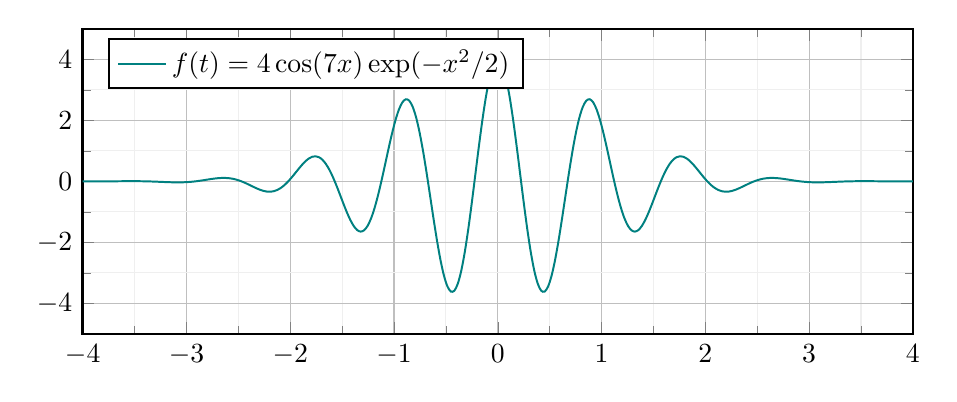
\begin{tikzpicture}
		\begin{axis}[
			grid = both,
			legend pos = north west,
			minor tick num = 1,
			major grid style = {lightgray},
			minor grid style = {lightgray!25},
			%title= {},
			width = \textwidth,
			height = 0.45 \textwidth,
			xmin=-4, xmax=4,
			ymin=-5, ymax=5,
			line width=0.3mm
			]
			
			\addplot[domain = -5:5,
			samples = 300,
			color = teal,
			smooth,
			line width = 0.025cm,] {4 * cos(7 * deg(x)) * e^(- (x^2) / 2)};
			
			\legend{$f(t) = 4 \cos(7x)\exp(-x^2 / 2)$};
		\end{axis}
	\end{tikzpicture}
	\caption{Построение wavelet Морле}
\end{figure}
В формализованном виде Wavelet преобразование имеет вид:
\begin{equation}
	\begin{split}
		f(t) & = \frac{1}{2\pi C_{\psi}} \int_{\R} \int_{\R} \frac{W_{\psi}(f_{a, b})}{a^2}\psi_{a, b}(t) \; da \; db\\
		C_{\psi} & = \int_{\R} \frac{|\hat{\phi}(\omega)|^2}{|\omega|} \; d \omega
	\end{split}
\end{equation}
Где $\hat{\phi}(\omega)$ - преобразование Фурье для выбранного в качестве основного Wavelet'а. А формула прямого перехода в пространство частоты и времени, то есть формула прямого Wavelet преобразования, имеет вид:
\begin{equation}
	W_{\psi}(f_{a, b}) = \frac{1}{\sqrt{a}}\int_{\R}f(t) \overline{\phi}\left( \frac{t - b}{a} \right) \; dt
\end{equation}
Где $b$ - параметр, отвечающий за сдвиг функции wavelet по сигналу, параметр $a$ - коэффициент сжатия/растяжения wavelet, а $\overline{\psi}$ - комплексное сопряжение.

Интересно, что отличия от преобразования Фурье минимальны, так как в преобразовании Wavelet просто взяты иные базисные функции, что сохраняет саму структуру действий при проведении подобного анализа. Поэтому все основные свойства, характерные для преобразования Фурье, остаются верными. Более подробно об этом в \cite{brunton2022data}. Графики, которые получаются после проведения данного анализа называются scalograms, что на русском скейлограммы. Далее приводим пример применения Wavelet анализа к показателям Apple.
\begin{figure}[H]
	\centering
	\includegraphics[width= 1.05\textwidth]{time frequency/scalogram_plots.png}
	\caption{График scalogram цены открытия и доходности Apple (IPO - 2022)}
	\label{fig::wavelet_example}
\end{figure}
Интересно, что теперь, по сравнению с анализом Фурье, четко выделено отсутствие какой-либо частотной информации для цен Apple, однако четко прослеживается очень большой ее объем в доходностях. Более того, наблюдая за негативными пиками в доходности, видим, что пики, падающие ниже $-20$ имеют четко выраженную лаговую структура. В верхней части scalogram для доходностей существуют яркие пики, которые аккурат влекут за собой падение доходности, что аналогично предыдущему подтверждает наличие частотной информации и доходностях акций.

Однако конкретно данный алгоритм, как и преобразование Фурье, не получится использовать для прогнозирования, таким образом, их (алгоритмов) главная задача в настоящей работе - обеспечение очистки данных от шумовых компонент, обусловленных как погрешностью, так и временным лагом между наблюдениями - в случае Apple - это примерно $35$ часов.

Теперь приводим пример работы алгоритма очистки посредством применения WA (Wavelet Analysis). Рассматриваем все ту же функцию (\myref{link::illustr_func}).
\begin{figure}[H]
	\centering
	\begin{tikzpicture}
		\begin{axis}[
			grid = both,
			legend pos = north west,
			minor tick num = 1,
			major grid style = {lightgray},
			minor grid style = {lightgray!25},
			%title= {},
			width = \textwidth,
			height = 0.45 \textwidth,
			xmin=-5, xmax=5,
			ymin=-4, ymax=7.5,
			line width=0.3mm
			]
			
			\addplot[color = orange, line width = 0.035cm] table [
			x=x, 
			y=y_clean, 
			col sep=comma,
			mark={},
			] {./source/source_csv/Illustration data/wavelet/wavelet_example_denoising.csv};
			
			\addplot[opacity = 0.25, color = blue] table [
			x=x, 
			y=y_initial, 
			col sep=comma,
			mark={},
			] {./source/source_csv/Illustration data/wavelet/wavelet_example_denoising.csv};
			
			\addplot[domain = -5:5,
			samples = 300,
			color = teal,
			smooth,
			line width = 0.025cm,] {sin(deg(5 * x)) + 1 / 4 * (x^2)};
			
			\legend{$f(x)$ очищенный, $f(x)$ c шумом, $f(x)$ без шума};
		\end{axis}
	\end{tikzpicture}
	\caption{Очистка ряда от шума посредством преобразования Wavelet}
\end{figure}
Ошибка RMSE$= 0.7649$, что заметно больше, что в случае применения метода MSSA, где ошибка $\text{RMSE} = 0.1744$ (\myref{link::mssa}). Таким образом, получается вывод, что для очистки от шума лучше использовать MSSA. Но в таком случае, появляется вопрос \textbf{Q}: Зачем весь этот метод тут, если, применяя его, не получается как прогнозировать (без специальных дополнительных предпосылок или теоретических выкладок, как, например, в статье \cite{schluter2010using}), так и лучше, чем MSSA очищать от шума (не строгое утверждение, а лишь основа на результате исследования настоящей работы)? \textbf{A}: Ответ присутствует в блоке (\myref{link::wavelet_nets}), где приводится описание применения Wavelet анализа к построению <<сетевых>> архитектур. Под <<сетевыми>> подразумеваются нейронные сети.

Таким образом, пока что вышеупомянутые методы Фурье и Wavelet преобразования остаются лишь прикладными к другим методам (это верно только для настоящей работы), так как напрямую для прогнозирования не применяются, однако это ничего не говорит об их качестве работы с анализируемыми данными. Далее переходим к описанию наиболее важной части текущего исследования, посвященной нейросетевому подходу к решению задачи прогнозирования показателей.
